\documentclass[a4paper,12pt]{article}
\usepackage{tabto}
\usepackage{amsmath}
\pagenumbering{gobble}
\usepackage{apacite}
\usepackage{pgfplots}
\usepackage{array}
\usepackage{caption}
\usepackage{graphicx}
\usepackage{float}
\usepackage{amssymb}
\usepackage{enumitem}
\usepackage{hyperref}

\begin{document}
	
\title{Data Integration\\Project report}
\author{Antoni Forzpanczyk and Jedrzej Szor}

\maketitle

\begin{abstract}
The report is a conclusion of work done to implement the practical assignment. In this document we will describe the wrappers used, the safety measures taken and the decisions made in order to provide a useful and secure application.
\end{abstract}

\section{Introduction}
The aim of that experiment is to familarize with the phenomenon of Hall effect. Hall effect appears in a conductor through which current is flowing, when placed in magnetic field. We examined dependence of Hall voltage on electric current, magnetic field and temperature. With the results we obtained during experiment, we could calculate Hall’s constant, charge carriers’ density and mobility as well as conductivity.
The report consists of three parts. First, in which we present a scheme of setup for analyzing Hall effect and give the method of measuring the Hall voltage. In the second part, we present the results of our measurements and calculations. The final part is a conclusion of our
analysis and calculations.

\newpage
\section{Measurement method}

\begin{table}[H]
\begin{center}
\caption{List of used symbols and corresponding quantities}
\begin{tabular}{|c|c|}
\hline
Symbol & Meaning\\
\hline
\hline
$I_p$ & Current\\
\hline
$U_H$ & Hall voltage\\
\hline
B & Magnetic induction\\
\hline
T & Temterature\\
\hline
I & Driving current\\
\hline
$R_H$ & Hall constant\\
\hline
e & Electron charge\\
\hline
l & Germanium sample length\\
\hline
a & Germanium sample width\\
\hline
d & Germanium sample thickness\\
\hline
p & Charge carriers' concentration\\
\hline
$\sigma$ & Conductivity\\
\hline
R & Sample resistance\\
\hline
$R_B$ & Sample resistance with B=0T\\
\hline
\end{tabular}
\end{center}
\end{table}


The setup consists of a power supply, teslameter,
electromagnet and the sample of p-germanium placed in its gap and a DMM which plays the role of voltmeter

The p-germanium sample used in the exercise is ? x ? x ? (\textbf{a x l x d} respectively),
has resistance R equal to R = ????? $\Omega$ and is placed on a plate in the gap of an electromagnet. \\

In the first measurement, the magnetic field B was constant and set to 300mT. We kept change the current starting at 0mA increasing it up to 40mA with a step of 5mA. Then we changed the direction of the current and measured Hall voltage again the same way with B = -300mT.\\

In the second measurement, the driving current Ip was constant and set to 30mA. We kept changing the magnetic field B starting from almost 0mT and increasing it up to 400mT simultaneously measuring the Hall voltage every 50mT. Then we changed the direction of the current and measured the Hall voltage the same way from 0mT up to -400mT.

Formula for the calculation of the Hall voltage:

\begin{equation}
U_h = \frac{1}{eq}jBa
\end{equation}

Where:
\begin{itemize}
\item $\frac{1}{eq} = R_H$ (Hall coefficient). \\The Hall coefficient can be used to determine the kind of
charge carriers.
\end{itemize}

Knowing the Hall coefficient we are capable of calculating the mobility  and concentration p of all carriers with the following formulas:

\begin{equation}
\mu = \sigma R_H
\end{equation}

\begin{equation}
p = \frac{1}{eR_H}
\end{equation}

The sample conductivity $\sigma$ can be computed with the knowledge of its its resistance and dimensions:

\begin{equation}
\sigma = \frac{l}{Rda}
\end{equation}

\newpage

\section{Results of our measurements}

Unfortunately, our measurements do not match to the characteristics of sample measurements. We were not able even conduct proper compputation based on that data. Based of agreement with supervisor we used data send by an email to compute desired results.

\begin{table}[H]
\begin{center}
\caption{Measurement of the Hall voltage $U_H$ with the respect to the current Ip flowing through the sample in constant magnetic field}
\begin{tabular}{|c|c|c|}
\hline
$I_p$[mA] & $U_H$[mV] & B[mT] \\   
\hline
\hline
0 &	3   & 300 \\
\hline
6 &	17  & 300 \\
\hline
10 &	24  & 300 \\
\hline
16 &	33  & 300 \\
\hline
19 &	38  & 300 \\
\hline
24 &	48  & 300 \\
\hline
30 &	56  & 300 \\
\hline
34 &	64  & 300 \\
\hline
40 &	74  & 300 \\
\hline
\end{tabular}
\end{center}
\end{table}


\begin{table}[H]
\begin{center}
\caption{Measurement of the Hall voltage $U_H$ with the respect to the current Ip flowing through the sample in constant magnetic field}
\begin{tabular}{|c|c|c|}
\hline
$I_p$[mA] & $U_H$[V] & B[mT] \\   
\hline
\hline
-40 &	-63  & 300 \\
\hline
-35 &	-54  & 300 \\
\hline
-30 &	-45  & 300 \\
\hline
-26 &	-39  & 300 \\
\hline
-20 &	-30  & 300 \\
\hline
-15 &	-19  & 300 \\
\hline
-10 &	-11  & 300 \\
\hline
-6 &	-4  & 300 \\
\hline
\end{tabular} 
\end{center}
\end{table}


\begin{table}[H]
\caption{Investigation of the Hall Voltage $U_H$ dependence on magnetic induction B in constant temperature T$\approx????^\circ C$ with constant driving current}
\begin{minipage}{.5\linewidth}
\centering
\begin{tabular}{|c|c|c|}
\hline
$I_p$[mA] & $U_H$[V] & B[mT] \\   
\hline
\hline
30    & 386	& 72\\
\hline
30    & 381	&	72\\
\hline
30    & 359	&	68\\
\hline
30    & 341	&	65\\
\hline
30    & 321	&	61\\
\hline
30    & 300	&	58\\
\hline
30    & 282	&	54\\
\hline
30    & 261	&	51\\
\hline
30    & 238	&	47\\
\hline
30    & 221	&	44\\
\hline
30    & 202	&	41\\
\hline
30    & 181	&	37\\
\hline
30    & 164	&	34\\
\hline
30    & 143	&	30\\
\hline
30    & 121	&	26\\
\hline
30    & 101	&	23\\
\hline
30    & 84	&	20\\
\hline
30    & 59	&	16\\
\hline
30    & 42	&	13\\
\hline
30    & 24	&	10\\
\hline
30    & 1	&	6\\
\hline

\end{tabular}
\end{minipage}%
\begin{minipage}{.5\linewidth}
\centering
\begin{tabular}{|c|c|c|}
\hline
$I_p$[mA] & $U_H$[V] & B[mT] \\   
\hline
\hline
30    & -26 &	1\\
\hline
30    & -44 &	-1\\
\hline
30    & -63 &	-4\\
\hline
30    & -83 &	-8\\
\hline
30    & -107 &	-12\\
\hline
30    & -121 &	-14\\
\hline
30    & -144 &	-18\\
\hline
30    & -163 &	-21\\
\hline
30    & -184 &	-25\\
\hline
30    & -205 &	-28\\
\hline
30    & -223 &	-31\\
\hline
30    & -246 &	-35\\
\hline
30    & -259 &	-37\\
\hline
30    & -278 &	-40\\
\hline
30    & -297 &	-43\\
\hline
30    & -323 &	-47\\
\hline
30    & -343 &	-50\\
\hline
30    & -361 &	-53\\
\hline
30    & -383 &	-57\\
\hline
30    & -398 &	-59\\
\hline
\end{tabular}
\end{minipage} 
\end{table}

\begin{figure} [p]
\begin{center}
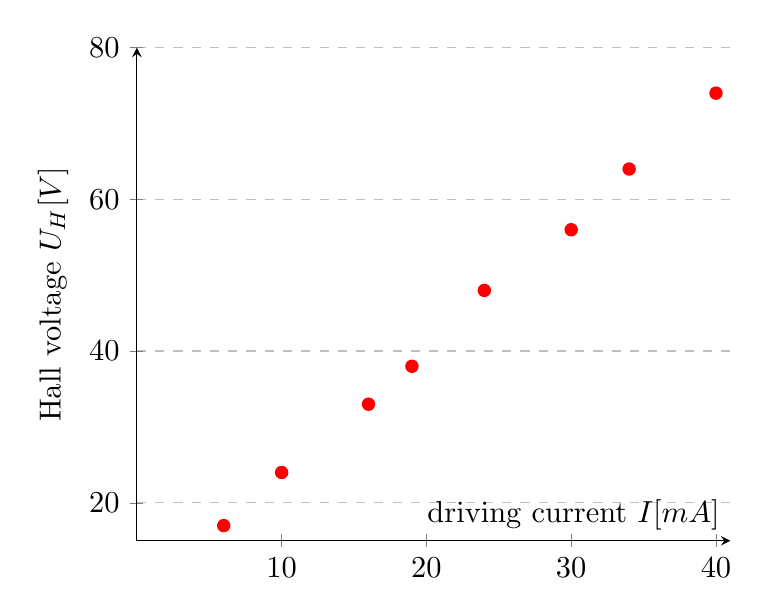
\begin{tikzpicture}[scale=1.1]
\begin{axis}[
xlabel={driving current $I[mA]$},
ylabel={Hall voltage $U_H[V]$},
xmin=0,xmax=41,
ymin=15,ymax=80,
ymajorgrids=true,grid style=dashed,
axis x line=center,
axis y line=left,
]

\addplot[color=red,mark=*,only marks]
coordinates {

(6,	17)
(10, 24)
(16	,33)
(19	,38)
(24	,48)
(30	,56)
(34	,64)
(40	,74)

};
\end{axis}

\end{tikzpicture}
\caption{Dependence of I on $U_H$ with constant B=300[mT]}
\end{center}
\end{figure}

\begin{figure} [p]
\begin{center}
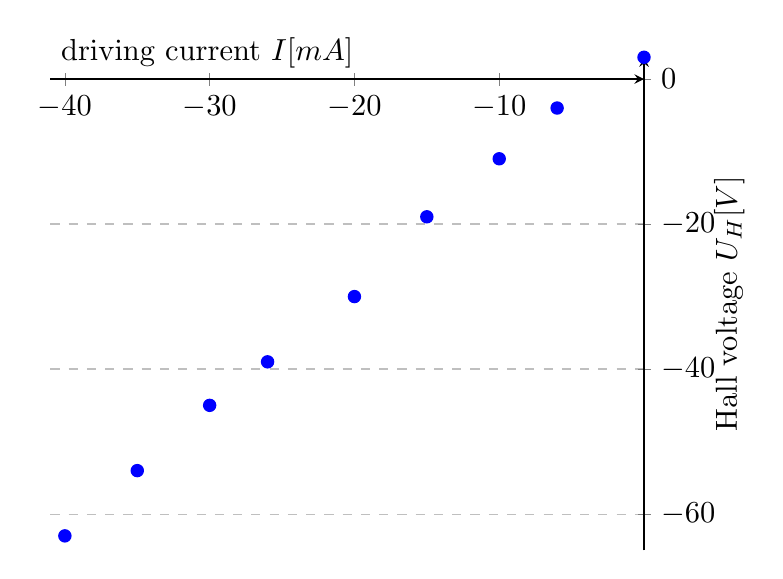
\begin{tikzpicture}[scale=1.1]
\begin{axis}[
xlabel={driving current $I[mA]$},
ylabel={Hall voltage $U_H[V]$},
xmin=-41,xmax=0,
ymin=-65,ymax=3,
ymajorgrids=true,grid style=dashed,
axis x line=center,
axis y line=right,
y label style={at={(1.1,0.5)}},
]

\addplot[color=blue,mark=*,only marks]
coordinates {

(-40,	-63)
(-35,	-54)
(-30,	-45)
(-26,	-39)
(-20,	-30)
(-15,	-19)
(-10,	-11)
(-6,	-4)
(0,		3)

};
\end{axis}

\end{tikzpicture}
\caption{Dependence of I on $U_H$ with constant B=300[mT]}
\end{center}
\end{figure}


\begin{figure} [H]
\begin{center}
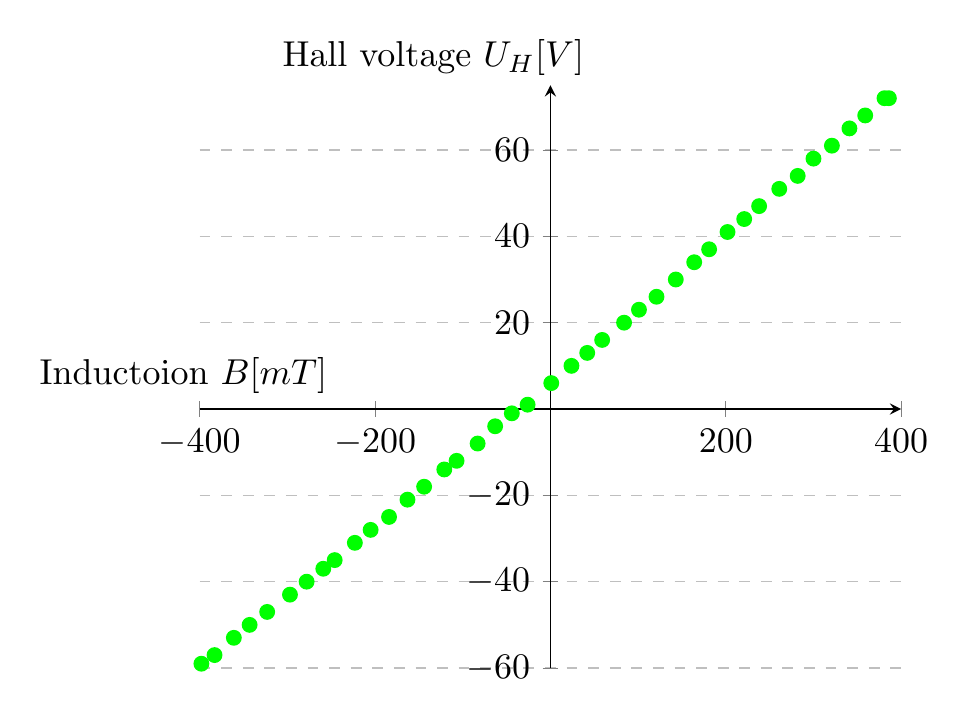
\begin{tikzpicture}[scale=1.3]
\begin{axis}[
axis x line=center,
axis y line=center,
xlabel={Inductoion $B[mT]$},
ylabel={Hall voltage $U_H[V]$},
xmin=-400,xmax=400,
ymin=-60,ymax=75,
ymajorgrids=true,
grid style=dashed,
y label style={at={(0.1,1.1)}},
x label style={at={(0.2,0.45)}}
]

\addplot[color=green,mark=*,only marks]
coordinates {

(386,	72)
(381,	72)
(359,	68)
(341,	65)
(321,	61)
(300,	58)
(282,	54)
(261,	51)
(238,	47)
(221,	44)
(202,	41)
(181,	37)
(164,	34)
(143,	30)
(121,	26)
(101,	23)
(84,	20)
(59,	16)
(42,	13)
(24,	10)
(1,		6)
(-26,	1)
(-44,	-1)
(-63,	-4)
(-83,	-8)
(-107,	-12)
(-121,	-14)
(-144,	-18)
(-163,	-21)
(-184,	-25)
(-205,	-28)
(-223,	-31)
(-246,	-35)
(-259,	-37)
(-278,	-40)
(-297,	-43)
(-323,	-47)
(-343,	-50)
(-361,	-53)
(-383,	-57)
(-398,	-59)
};
\end{axis}

\end{tikzpicture}
\caption{Dependence of B on $U_H$ with constant I=30[mA]}
\end{center}
\end{figure}

Slope coefficient a, its error $\Delta$a were determined using the least square method:

\begin{equation*}
a = 0,1683 \pm 0,0005
\end{equation*}

Calculating Hall constant:
\begin{equation*}
-
\end{equation*}

Calculating concentration of charge carriers:
\begin{equation*}
-
\end{equation*}

Calculating the conductivity $\sigma$:
\begin{equation*}
-
\end{equation*}

Calculating the mobility $\mu$ of the carriers:
\begin{equation*}
-
\end{equation*}

\begin{figure} [H]
\begin{center}
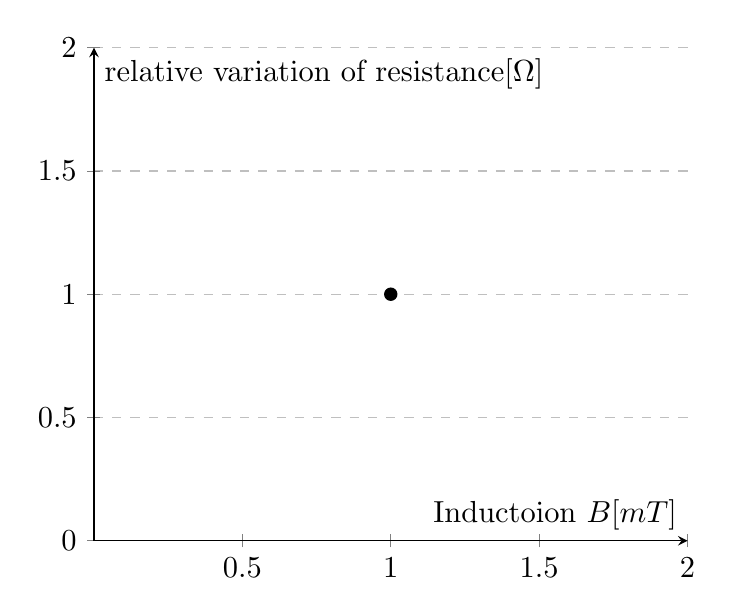
\begin{tikzpicture}[scale=1.1]
\begin{axis}[
axis x line=center,
axis y line=center,
xlabel={Inductoion $B[mT]$},
ylabel={relative variation of resistance$[\Omega]$},
xmin=0,xmax=2,
ymin=0,ymax=2,
ymajorgrids=true,
grid style=dashed,
axis x line=center,
axis y line=left,
]

\addplot[color=black,mark=*,only marks]
coordinates {
(1,1)
};
\end{axis}
\end{tikzpicture}
\caption{The relative variation of resistance $\frac{R-R_B}{R}$ plotted on magnetic induction B}
\end{center}
\end{figure}

\section{Conclusions}

\section{References}
\begin{enumerate}[label={[\arabic*]}]
\item Perfect raport: \url{https://ftims.edu.p.lodz.pl/pluginfile.php/94757/mod_resource/content/1/perfect_report.pdf}
\item Excercise procedure D-80: \url{https://ftims.edu.p.lodz.pl/mod/resource/view.php?id=42953}
\end{enumerate}

\end{document}